\documentclass{standalone}
\usepackage{tikz}
\usepackage{verbatim}
\usepackage{latexsym}
\usetikzlibrary{positioning}
\begin{document}
\pagestyle{empty}
  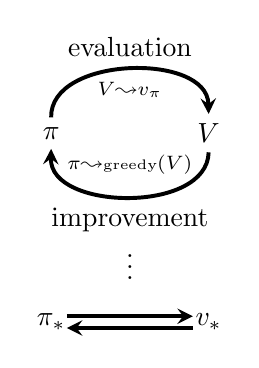
\begin{tikzpicture}
    \node (pi) at (-1, 0) {$\pi$};
    \node (v)  at ( 1, 0) {$V$};
    \path[-stealth, line width=0.5 mm] (pi) edge[bend left = 90] (v);
    \path[-stealth, line width=0.5 mm] (v)  edge[bend left = 90] (pi);
    \node at (0, 1.1) {evaluation};
    \node at (0, 0.55) {$\scriptstyle V \leadsto v_\pi$};
    \node at (0, -0.4) {$\scriptstyle \pi \leadsto \textrm{\tiny greedy}(V)$};
    \node at (0, -1.1) {improvement};
    \node at (0, -1.6) {$\vdots$};
    \node (pistar) at (-1, -2.4) {$\pi_*$};
    \node (pistar) at (1, -2.4) {$v_*$};
    \draw[-stealth, line width=0.5 mm] (-.8, -2.325) -- (.8, -2.325);
    \draw[stealth-, line width=0.5 mm] (-.8, -2.475) -- (.8, -2.475);
  \end{tikzpicture}
\end{document}